\documentclass[aspectratio=169]{beamer}

\usepackage{ccicons}
\usepackage{fontspec}
\usepackage{listings}
\usepackage{tikz}
\usepackage{svg}

\definecolor{uclablue}{RGB}{39,116,174}
\definecolor{uclagold}{RGB}{255,179,0}

\definecolor{ubcorange}{RGB}{158, 66, 37}

\definecolor{cugold}{RGB}{207, 184, 124}
\definecolor{cudarkgray}{RGB}{86, 90, 92}

\definecolor{solarizedred}{RGB}{220, 50, 47}
\definecolor{solarizedblue}{RGB}{38, 139, 210}
\definecolor{solarizedgreen}{RGB}{133, 153, 0}
\definecolor{solarizedpurple}{RGB}{108, 113, 196}
\definecolor{solarizedmagenta}{RGB}{211, 54, 130}

\definecolor{pantone655}{RGB}{0, 42, 92}
\definecolor{pantone7453}{RGB}{123, 164, 217}
\definecolor{pantone633}{RGB}{0, 139, 176}
\definecolor{pantone7492}{RGB}{218, 229, 205}

\colorlet{primarycolor}{pantone655}
\colorlet{secondarycolor}{pantone7453}


\usetikzlibrary{
  arrows,
  arrows.meta,
  automata,
  backgrounds,
  calc,
  chains,
  decorations.pathreplacing,
  fit,
  intersections,
  matrix,
  overlay-beamer-styles,
  positioning,
  shapes,
  shapes.multipart,
  tikzmark,
}
\usetikzmarklibrary{listings}

\hypersetup{
  colorlinks=true,
  urlcolor=cudarkgray,
}

\setbeamercolor{frametitle}{fg=primarycolor}
\setbeamercolor{structure}{fg=primarycolor}
\setbeamercolor{enumerate item}{fg=black}
\setbeamercolor{itemize item}{fg=black}
\setbeamercolor{itemize subitem}{fg=black}

\setbeamersize{text margin left=26.6mm}
\addtolength{\headsep}{2mm}

\setbeamertemplate{navigation symbols}{}
\setbeamertemplate{headline}{}
\setbeamertemplate{footline}{}
\setbeamertemplate{itemize item}{\color{black}}
\setbeamertemplate{itemize items}[circle]

\setbeamertemplate{footline}{
  \begin{tikzpicture}[remember picture,
                      overlay,
                      shift={(current page.south west)}]
    \node [black!50, inner sep=2mm, anchor=south east]
          at (current page.south east) {\footnotesize \insertframenumber};
  \end{tikzpicture}
}

\setsansfont{Inter}[Scale=MatchLowercase]
\setmonofont{Hack}[Scale=MatchLowercase]

\makeatletter
\newcommand\version[1]{\renewcommand\@version{#1}}
\newcommand\@version{}
\def\insertversion{\@version}

\newcommand\lecturenumber[1]{\renewcommand\@lecturenumber{#1}}
\newcommand\@lecturenumber{}
\def\insertlecturenumber{\@lecturenumber}
\makeatother

\setbeamertemplate{title page}
{
  \begin{tikzpicture}[remember picture,
                      overlay,
                      shift={(current page.south west)},
                      background rectangle/.style={fill=pantone655},
                      show background rectangle]
    \node [anchor=west, align=left, inner sep=0, text=white]
          (lecturenumber) at (\paperwidth / 6, \paperheight * 3 / 4)
          {\Large Lecture \insertlecturenumber};
    \node [inner sep=0, align=left, text=white, node distance=0,
          above left=of lecturenumber, anchor=south west, yshift=2mm]
          {\Large ECE 344: Operating Systems};
    \node (title) [inner sep=0, anchor=west, align=left, text=white,
                   text width=30em]
          at (\paperwidth / 6, \paperheight / 2)
          {{\bfseries \Huge \inserttitle{}}};
    \node [inner sep=0, align=right, text=white, node distance=0,
          below right=of title, anchor=north east, yshift=-1mm]
          {{\footnotesize \ttfamily \insertversion}};
    \node [inner sep=0, text=white, align=left, anchor=west]
          (author) at (\paperwidth / 6, \paperheight / 4)
          {\insertauthor};
    \node [text=white, inner sep=0, align=left, node distance=0,
           below left=of author, anchor=north west, yshift=-2mm]
          {\insertdate};
    \node [align=right, anchor=south east, inner sep=2mm, text=white]
          (license) at (\paperwidth, 0)
          {\footnotesize This  work is licensed under a
           \href{http://creativecommons.org/licenses/by-sa/4.0/}
                {\color{pantone7453} Creative Commons Attribution-ShareAlike 4.0
                 International License}};
    \node [text=white, inner sep=0, align=right, node distance=0,
           above right=of license, anchor=south east, xshift=-2mm]
          {\Large \ccbysa};
  \end{tikzpicture}
}

\tikzset{
  >=Straight Barb[],
  shorten >=1pt,
  initial text=,
}

\lstset{
  basicstyle=\footnotesize\ttfamily,
  language=C,
  escapechar=@,
  commentstyle=\color{black!50},
}


\lecturenumber{3}
\title{Process Life Cycle}
\version{1.1.0}
\author{Jon Eyolfson}
\date{September 13/14, 2022}

\begin{document}
  \begin{frame}[plain, noframenumbering]
    \titlepage
  \end{frame}

  \begin{frame}
    \frametitle{A Process is an Instance of a Running Program}

    A \textit{program} (or application) is just a static definition, including:

    \begin{itemize}
      \item Instructions
      \item Data
      \item Memory allocations
      \item Symbols it uses
    \end{itemize}

    \vspace{2em}

    A \textit{process} executes a program, and the kernel manages processes
  \end{frame}

  \begin{frame}
    \frametitle{Process is like a Combination of all the Virtual Resources}

    If we consider a ``virtual CPU'', the OS needs to track all registers

    \vspace{2em}

    It also contains all other resources it can access (memory and I/O)

    \vspace{4em}

    Every execution runs the same code (part of the program)

    \hspace{2em} An execution is running some specific code (part of the
                 process)
  \end{frame}

  \begin{frame}
    \frametitle{A Process is More Flexible}

    A process contains both the program and information specific
    to its execution

    \vspace{4em}

    It allows multiple executions of the same program

    \vspace{2em}

    It even allows a process to run multiple copies of itself
  \end{frame}

  \begin{frame}
    \frametitle{A Process Control Block (PCB) Contains All Execution Information}


    Specifically, in Linux, this is the \texttt{\color{primarycolor}
    task\_struct} you can browse on
    \href{https://github.com/torvalds/linux/blob/master/include/linux/sched.h\#L727}
         {GitHub}

    \vspace{2em}

    It contains:
    \begin{itemize}
      \item Process state
      \item CPU registers
      \item Scheduling information
      \item Memory management information
      \item I/O status information
      \item Any other type of accounting information
    \end{itemize}
  \end{frame}

  \begin{frame}
    \frametitle{Aside: Concurrency and Parallelism Aren't the Same}

    Concurrency

    \hspace{2em} Switching between two or more things (can you get interrupted)

    \hspace{4em} Goal: make progress on multiple things

    \vspace{4em}

    Parallelism

    \hspace{2em} Running two or more things at the same time (are they independent)

    \hspace{4em} Goal: run as fast as possible
  \end{frame}

  \begin{frame}
    \frametitle{A Real Life Situation of Concurrency and Parallelism}


    You're sitting at a table for dinner, and you can:
    \begin{itemize}
      \item Eat
      \item Drink
      \item Talk
      \item Gesture
    \end{itemize}
    You're so hungry that if you start eating you won't stop until you finish

    \vspace{4em}

    Which tasks can and can't be done concurrently, and in parallel?
  \end{frame}

  \begin{frame}
    \frametitle{Choose Any Two Tasks in the Real Life Example}

    You can't eat and talk (or drink) at the same time, and you can't switch

    \hspace{2em} Not parallel and not concurrent

    \vspace{2em}

    You could eat and gesture at the same time, but you can't switch

    \hspace{2em} Parallel and not concurrent

    \vspace{2em}

    You can't drink and talk at the same time, and you could switch

    \hspace{2em} Not parallel and concurrent

    \vspace{2em}

    You can talk (or drink) and gesture at the same time, and you could switch

    \hspace{2em} Parallel and concurrent
  \end{frame}


  \begin{frame}
    \frametitle{Uniprogramming is for Old Batch Processing Operating Systems}

    Uniprogramming: only one process running at a time

    \hspace{2em} Two processes are not parallel and not concurrent, no matter what

    \vspace{2em}

    Multiprogramming: allow multiple processes

    \hspace{2em} Two processes can run in parallel or concurrently

    \vspace{4em}

    Modern operating systems try to run everything in parallel and concurrently
  \end{frame}

  \begin{frame}
    \frametitle{Process State Diagram (You Could Rename Waiting to Ready)}

    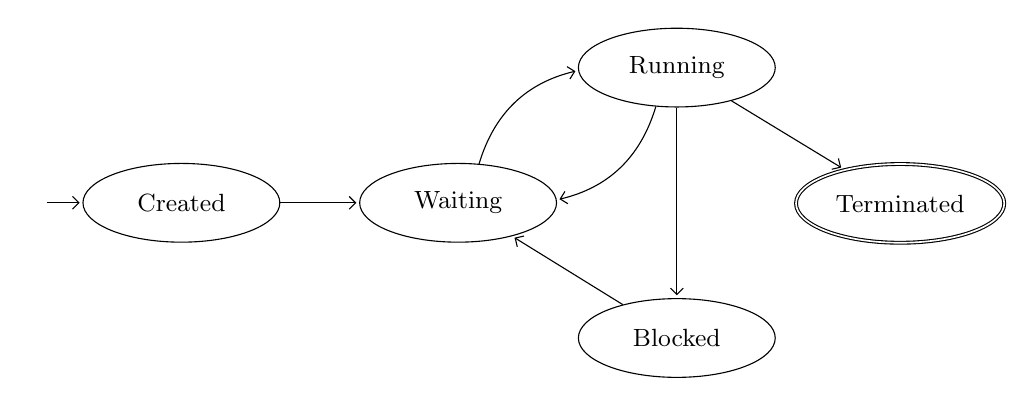
\begin{tikzpicture}[
      every state/.style={ellipse, minimum width=2.5cm, minimum height=1cm, font=\small},
    ]
      \node [state, initial] (created) {Created};
      \node [state, right=of created] (waiting) {Waiting};
      \node [state, above right=of waiting] (running) {Running};
      \node [state, below right=of waiting] (blocked) {Blocked};
      \node [state, accepting, below right=of running] (terminated) {Terminated};
      \path [->] (created) edge (waiting)
                 (waiting) edge [bend left] (running)
                 (running) edge [bend left] (waiting)
                 (running) edge (blocked)
                 (blocked) edge (waiting)
                 (running) edge (terminated);
    \end{tikzpicture}
  \end{frame}

  \begin{frame}
    \frametitle{The Scheduler Decides When To Switch}

    To create a process, the operating system has to at least load it into memory

    \hspace{2em}

    When it's waiting, the scheduler (coming later) decides when it's running

    \hspace{2em}

    We're going to first focus on the mechanics of switching processes
  \end{frame}

  \begin{frame}
    \frametitle{The Core Scheduling Loop Changes Running Processes}

    \begin{enumerate}
      \item Pause the currently running process 
      \item Save its state, so you can restore it later
      \item Get the next process to run from the scheduler
      \item Load the next process' state and let that run
    \end{enumerate}
  \end{frame}

  \begin{frame}
    \frametitle{We Can Let Processes Themselves, or the Operating System Pause}
    
    Cooperative multitasking

    \hspace{2em} The processes use a system call to tell the operating system to
    pause it

    \vspace{2em}

    True multitasking

    \hspace{2em} The operating system retains control and pauses processes

    \vspace{4em}

    For true multitasking the operating system can:

    \begin{itemize}
      \item Give processes set time slices
      \item Wake up periodically using interrupts to do scheduling
    \end{itemize}
  \end{frame}

  \begin{frame}
    \frametitle{Swapping Processes is called Context Switching}

    We've said that at minimum we'd have to save all of the current registers

    \hspace{2em} We have to save all of the values, using the same CPU as we're
    trying to save

    \vspace{2em}

    There's hardware support for saving state, however you may not want to save
    everything

    \vspace{2em}

    Context switching is pure overhead, we want it to be as fast as possible


    \vspace{4em}

    Usually there's a combination of hardware and software to save as little as
    possible
  \end{frame}

  \begin{frame}
    \frametitle{System Calls are Rare in C}

    Mostly you'll be using functions from the C standard library instead

    \vspace{2em}

    Most system calls have corresponding function calls in C, but may:
    \begin{itemize}
      \item Set \texttt{errno}
      \item Buffer reads and writes (reduce the number of system calls)
      \item Simplify interfaces (function combines two system calls)
      \item Add new features
    \end{itemize}
  \end{frame}

  \begin{frame}[fragile]
    \frametitle{C \texttt{exit} Has Additional Features}

    System call \texttt{exit} (or \texttt{exit\_group}): the program
    stops at that point

    \vspace{1em}

    C \texttt{exit}: there's a feature to register functions to call
    on program exit (\texttt{atexit})

    \vspace{1em}

    \begin{lstlisting}[xleftmargin=2em]
#include <stdio.h>
#include <stdlib.h>

void fini(void) {
  puts("Do fini");
}

int main(int argc, char **argv) {
  atexit(fini);
  puts("Do main");
  return 0;
}
    \end{lstlisting}
    \vspace{-1em}
    \begin{flushright}
      \lstinline|lecture-03/atexit-example|
    \end{flushright}
  \end{frame}

  \begin{frame}
    \frametitle{\texttt{execve} Replaces the Process with Another Program, and Resets}

    \texttt{execve} has the following API:
    \begin{itemize}
      \item \texttt{pathname}: Full path of the program to load
      \item \texttt{argv}: Array of strings (array of characters), terminated by a null pointer

            \hspace{2em} Represents arguments to the process
      \item \texttt{envp}: Same as \texttt{argv}

            \hspace{2em} Represents the environment of the process
      \item Returns an error on failure, does not return if successful
    \end{itemize}
  \end{frame}

  \begin{frame}[fragile]
    \frametitle{\texttt{execve-example.c} Turns the Process into \texttt{ls}}

    \begin{lstlisting}
int main(int argc, char *argv[]) {
  printf("I'm going to become another process\n");
  char *exec_argv[] = {"ls", NULL};
  char *exec_envp[] = {NULL};
  int exec_return = execve("/usr/bin/ls", exec_argv, exec_envp);
  if (exec_return == -1) {
    exec_return = errno;
    perror("execve failed");
    return exec_return;
  }
  printf("If execve worked, this will never print\n");
  return 0;
}
    \end{lstlisting}
  \end{frame}

  \begin{frame}
    \frametitle{The Operating System Creates and Runs Processes}

    The operating system has to:
    \begin{itemize}
      \item Loads a program, and create a process with context
      \item Maintain process control blocks, including state
      \item Switch between running processes using a context switch
      \item Replace programs running in processes (Unix)
    \end{itemize}
  \end{frame}



\end{document}
